\cleartooddpage[\thispagestyle{empty}]
\chapter{The Dark Matter Paradigm}\label{ch_dm}

  Dark matter makes up 26.5\% of the universe's energy and 81.5\% of its mass~\cite{planck2015}.
  It has had a significant impact on the development of the universe, shaping its present day distribution.
  This chapter discusses the main features of Dark Matter physics.
  These include the astrophysical evidence for the existance of Dark Matter, an outline of the current cosmological paradigm of $\Lambda$CDM and the Standard Model, as well as arguments for why Dark Matter may be in the form of a new, unknown particle.

  %From: https://arxiv.org/abs/1502.01589 , Table 3, column [4] :
  %  omega_b h^2 = 0.02225
  %  omega_c h^2 = 0.1198
  %  H_0         = 67.27 km / s / Mpc
  %  h           = H_0 / ( 100 km / s / Mpc ) = 0.6727
  %thus:
  %  omega_b = 0.02225 / h^2 = 0.0491 =  4.9% of universe's energy is in baryonic matter
  %  omega_c = 0.1198  / h^2 = 0.2647 = 26.5% of universe's energy is in dark matter
  %  ( 26.5 - 4.9 ) / 26.5 = 81.5% of universe's mass is stored in dark matter

\section{Astrophysical Evidence for Dark Matter}
  
  The current effects attributed to Dark Matter can be grouped into three observable physical effects, and four different length scales.
  These physical effects include observations of gravity pulling on electromagnetic emitters, gravity bending background light, and the universe's total energy budget.
  On the smallest length scales, concentrations of several thousand stars can be seen revolving around their center of mass, at a larger distribution of speeds than one would expect from the existing visible amount of matter.
  At larger scales the optical light from galaxies, as well as hydrogen lines, can be used to measure the amount of mass and its rotational velocity around the center of galaxies.
  At even larger scales, galaxy velocities can be measured and compared, x-ray telescopes can monitor the amount of hot gas, and mass-heavy areas of space will gravitationally lens background galaxies.
  At the the largest scale, the measurement of oscillations in the cosmic microwave background can be used to determine the amount of dark and baryonic matter.
  
  \subsection{Scales of $10^{19}\:\text{m}$ : Dwarf Galaxies}\label{dm_dwarfscale}
    % 10^19m comes from: 
    % fornax dwarf spheroidal galaxy wiki page
    %    17' x 12.6' in solid angle, call it 15'
    %    140kpc away  
    %    140kpc * Tan(15') = 0.6kpc = 1.8*10^19m ~ 10^19m
    At scales of $\nicetilde 10^{19}$m, groups of thousands stars, called satellite galaxies or dwarf galaxies, lie at the edge of full size galaxies like our own.
    These dwarf galaxies are strong evidence for dark matter because their luminous matter is not enough to gravitationally bind them.
    An example of a dwarf galaxy is shown in Figure~\ref{fig:sculptor}, the Sculptor Dwarf Galaxy, imaged in the optical frequencies by the MPG/ESO Telescope.
    \begin{figure}[ht]
      \centering
      \includegraphics[width=0.9\textwidth]{images/sculptor/sculptor.eps}
      \caption[Sculptor Dwarf Galaxy]{
        The Sculptor Dwarf Galaxy \cite{sculptor_image}, imaged with the MPG/ESO telescope~\cite{sculptor_paper}.
        This dwarf galaxy has a $\frac{M_\odot}{L_\odot}$ ratio of 15.3~\cite{sculptor_ml}.
      }
      \label{fig:sculptor}
    \end{figure}

    Measuring the mass of these dwarf galaxies is done in two ways.
    In the first, telescopes observed the individual spectra of these stars, allowing for their line-of-sight velocity to be calculated~\cite{dwarf_gal_red_giant}.
    The width of the distribution of the velocities is called the velocity dispersion.
    By looking at this velocity dispersion, the total mass of the dwarf galaxy can be inferred~\cite{dwarf_gal_vel_dispersion, dwarf_gal_vel_dispersion2}.
    What makes this possible is that the velocity dispersion of a group of stars is proportional to the total mass of the graviational well.
    This can be seen by applying the virial theorem and Maxwell-Boltzmann statistics.
    The virial theorem, Equation~\ref{eqn:virial}, states an n-body system in equilibrium will always have the same ratio of kinetic energy (KE) to potential energy (PE).
    \begin{equation}\label{eqn:virial}
      2 \text{KE} = \text{PE}
    \end{equation}
    Thus, by measuring stellar velocities and calculating the total kinetic energy of a group of stars, the potential energy can be calculated, which indicates the amount of mass present in the group.

    % derivation from https://en.wikipedia.org/wiki/Maxwell%E2%80%93Boltzmann_distribution
    Maxwell-Boltzmann statistics can also be used to measure the amount of mass in a system.
    Using the Maxwell-Boltzmann distribution, the velocity probability density function is then Equation~\ref{eqn:mb_vel3d}:
    \begin{equation}\label{eqn:mb_vel3d}
      f_v(v_x,v_y,v_z)= \left ( \frac{m}{2\pi k T} \right ) ^ { \frac{3}{2} } \text{exp} \left [ - \frac{m \left ( v_x^2 + v_y^2 + v_z^2 \right )}{2 k T} \right ]
    \end{equation}
    where $m$ is the mass of the system, $k$ is the Boltzmann constant, and $T$ is the equilibrium temperature of the system {\color{red}(??)}.
    
    In one dimension, each velocity distribution is a normal distribution, described by Equation~\ref{eqn:mb_vel1d},
    \begin{equation}\label{eqn:mb_vel1d}
      f_v(v_i) = \sqrt{ \frac{m}{2\pi k T} } \text{exp} \left [ - \frac{m v_i^2}{2kT} \right ]
    \end{equation}
    where the mean velocity in each direction is $\mu_{v_i} = 0$ and the standard deviation is $\sigma_{v_i} = \sqrt{\frac{kT}{m}}$.
    When these three dimensions are combined into a 3-dimensional normal distribution, the mean velocity vector is $\vec{\mu}_v = \vec{0}$, and its distribution has a width described by Equation~\ref{eqn:mb_sigma}:
    \begin{equation}\label{eqn:mb_sigma}
      \sigma_v = \sqrt{\frac{3kT}{m}}
    \end{equation}
    A Maxwell-Boltzmann distribution's most probable speed is $\left \langle v \right \rangle = \frac{2}{\sqrt{\pi}} \sqrt{\frac{2kT}{m}}$.
    Therefore, measuring the mean speed and distribution of speeds of a group of stars can yield the total mass of the system, described by Equation (??).
    {\color{red}(THIS MAXWELL STUFF IS WRONG, THE MASS $m$ CANCELS, NEEDS TO BE REDONE!??)}
    
    Thus, by measuring the distribution of star velocities and the average temperature of the system {\color{red}(what is temp T of the system??  does it come from $v_p$??  clean up this paragraph??)}, the total mass of a system can be calculated: $m = \frac{3kT}{\sigma^2}$.
    As stellar velocity measurements rely on doppler-shifted spectral lines, and not the star's absolute brightness, any derived mass estimates are fairly resistant to changes in observed brightness.
    These changes in brightness can be from atmospheric variations during telescope observations or changes in the amount of light-absorbing dust in the line-of-sight.

    The second way to measure galaxy masses is by measuring the total brightness of a galaxy, and divide by the luminosity of the Sun $L_\odot$.
    This then indicates the number of solar masses $M_\odot$ contained in the galaxy, a measure of its baryonic (i.e. 'bright', not dark) mass.
    For these conversions, nominal values are $M_\odot =$ \SI{1.9885e30}{kg} and $L_\odot =$ \SI{3.828e26}{W}, though different authors may use slightly different values depending on the year of publication~\cite{iau_solarconstants}.
    % from https://arxiv.org/pdf/1510.07674.pdf
    % L_\odot from page 3, table "SOLAR CONVERSION CONSTANTS" 
    % M_\odot :
    %   G*M_\odot = 1.3271244e20 m^3 s^-2 (from table "SOLAR CONVERSION CONSTANTS")
    %   G = 6.67408e-11 m^3 kg^-1 s^-2
    %   thus 
    %   M_\odot = 1.3271244e20 m^3 s^-2 / 6.67408e-11 m^3 kg^-1 s^2
    %           = 1.98847e30 kg
    
    The first way measures the 'total' mass from the rotational profile, while the second only measures the mass of its 'luminous' parts.
    The ratio of the 'total' mass divided by the 'luminous' mass is called the mass-to-light ratio, which indicates the amount of Dark Matter present in the galaxy~\cite{faber_ml}.
    Dwarf galaxies have mass-to-light ratios of around 5-100 $\frac{M_\odot}{L_\odot}$, but can reach up to \nicetilde 1000~\cite{Simon2007_dwarfgalaxykeck}.
    These high values are considered strong evidence in favor of Dark Matter.
    A random assortment of Local Group dwarf galaxies and their $\frac{M_\odot}{L_\odot}$ is shown in Table~\ref{tab:mlratios:dwarfgals}.
    
    \begin{table}[]
      \centering
      \caption{$\frac{M_\odot}{L_\odot}$ ratios of various dwarf galaxy objects~\cite{localdwarfs}.}
      \label{tab:mlratios:dwarfgals}
      \begin{tabular}{l r}
        Object      &  Mass, units of $\frac{M_\odot}{L_\odot}$ \\
        \hline
        IC 10       &  0.1 \\
        NGC 147     &  7.1 \\
        NGC 185     &  2.5 \\
        NGC 205     & 12   \\
        LGS 3       & 21   \\
        IC 1613     &  1.4 \\
        Carina      & 30   \\
        Antlia      &  7.4 \\
        Leo I       &  3.1 \\
        Sextans     & 34   \\
        Ursa Minor  & 60   \\
        Draco       & 58   \\
        Sagittarius & 22   \\
      \end{tabular}
    \end{table}
    
    As an additional piece of evidence for Dark Matter, dwarf galaxies near the Perseus cluster were studied.
    From the gravitational potential of their baryonic mass alone, these dwarf galaxies should be ripped apart by the tidal disruption of the Perseus cluster.
    Instead, observations of these dwarf galaxies indicate they remain intact, leading to the conclusion that the presence of Dark Matter is providing extra gravitational force~\cite{Penny2009}.
    
    \FloatBarrier

  \subsection{Scales of $10^{20}\:\text{m}$ : Galaxies}\label{dm_gal}
    %
    % galaxy rotation curve wiki page, M33 has curve measurements out to 50,000ly
    %   50,000ly = 4.7*10^20m ~ 10^20m
    At scales of $\nicetilde 10^{20}$m, the effects of Dark Matter on galaxies are observable.
    Within galaxies, the amount of light observed in a sector predicts a lower amount of mass, while observing the line-of-sight velocity predicts a higher amount of mass.
    
    In the first prediction technique, the total amount of light produced by a quadrant of a galaxy is measured with optical telescopes.
    Then, as in Section~\ref{dm_dwarfscale}, the amount of light produced can be compared with the Sun as a standard mass-to-light ratio, allowing for a prediction of the amount of mass contained in that sector.
    Known mass-to-light ratios can then be used to calculate the total amount of mass within that quadrant.
    For example, in a survey of 25 galaxies in Ref. \cite{galaxy_mass_light_ratio}, most possesed a mass-to-light ratio of 1 to 10.

    In the second prediction technique, a galaxy's emission spectrum is observed at many positions around its disk (center, outer edges, etc).
    By comparing the orientation of the disk with the doppler-shifted position of well-known spectral lines, one can calculate the average velocity that each section is traveling at around the center of its galaxy, forming a rotation curve~\cite{rotation_curve_review,spiral_galaxy_rot_curve,milkyway_dm_evidence}.
    Newton's law of gravity can then be used to calculate the mass contained within a sphere of that same radius.
    This calculation results in a larger amount of mass than the one found simply from the total amount of light observed.
    
    In Figure~\ref{fig:m33rotcurve}, a rotation curve from M33 observations is shown.
    The observed velocity curve (the datapoints) continues to increase at larger radii.
    If the galaxy was only made of stars, then the rotation curve would follow the short dashed line.
    If the galaxy was only made of gas, then the rotation curve would instead follow the long dashed line.
    As these two major components do not combine to form the observed rotation curve, the presence of Dark Matter can account for the difference, shown as the dashed-dotted line~\cite{m33rotcurve}.
    
    \begin{figure}[ht]
      \includegraphics[width=0.9\textwidth]{images/m33rotcurve/m33rotcurve.eps}
      \caption[M33 Rotation Curve]{
        The rotation curve from M33~\cite{m33rotcurve}.
        The solid line is the best fitting model to the observed velocity measurments.
        The short dashed line is the stellar disk contribution, the gas contribution is the long dashed line, and the dashed-dotted line is the Dark Matter contribution.
      }
      \label{fig:m33rotcurve}
    \end{figure}
    
    \begin{table}[]
      \centering
      \caption{$\frac{M_\odot}{L_\odot}$ ratios of various galactic-scale objects~\cite{faber_ml}.}
      \label{tab:mlratios}
      \begin{tabular}{l r}
        Object          & Mass, units of $\frac{M_\odot}{L_\odot}$ \\
        \hline
        M31 (Andromeda) &  7.6  \\
        M33             &  4.5  \\
        M51             &  3.3  \\
        M81             &  8.5  \\
        NGC 801         &  2.4  \\
        NGC 2403        &  5.5  \\
        NGC 2841        & 10.6  \\
        NGC 4324        &  5.5  \\
        NGC 6822        &  0.58 \\
      \end{tabular}
    \end{table}
      
    A random sample of galaxies from Ref. \cite{faber_ml} are shown alongside their mass-to-light ratios in Table \ref{tab:mlratios}.
    Our own Milky Way galaxy is measured to have a mass to light ratio of \SIrange{1.2}{1.5} $\frac{M_{\odot}}{L_{\odot}}$~\cite{milkyway_ml_ratio}, indicating for every 5 sun-like stars in our galaxy, there are another two stars worth of dark matter.
    
    The further evidence of dark matter can also be deduced through additional weak gravitational lensing~\cite{weak_lensing_2001}.
    Lensing of elliptical galaxies can constrain mass profiles~\cite{weak_lensing_ellipse}.{\color{red}(expand??)}
    \begin{figure}
      \centering
      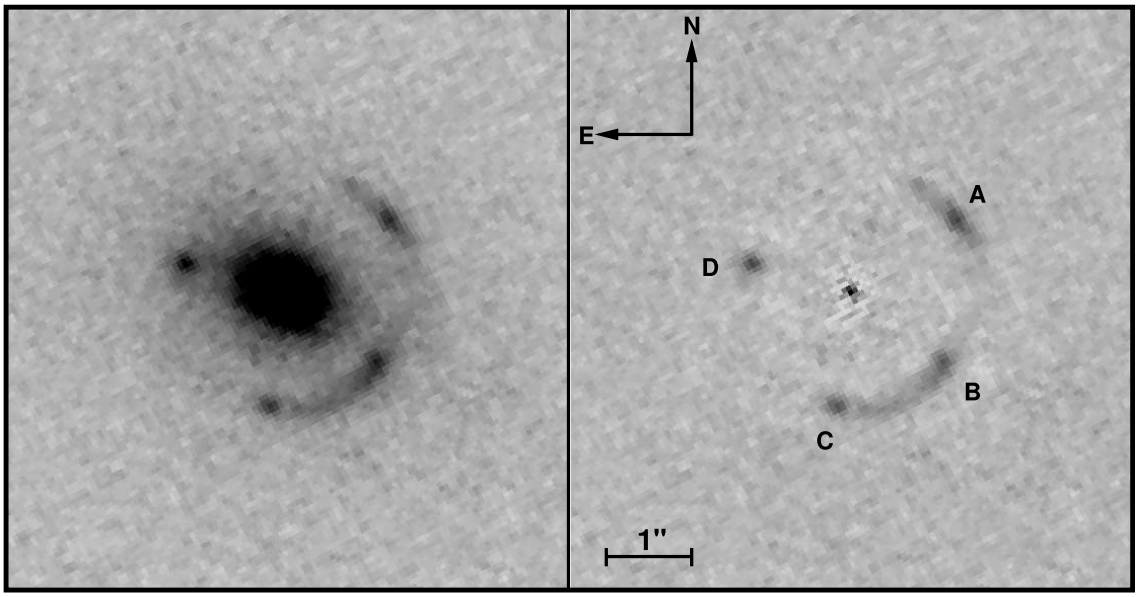
\includegraphics[width=0.95\textwidth]{images/weak_lensing_ellipse/weak_lensing.pdf}
      \caption[Weak Lensing with an Ellipse Galaxy]{
        Galaxy 0047-281 imaged by the Hubble Space Telescope, from Ref. \cite{weak_lensing_ellipse}.
        Left: Original image.
        Right: Same as Left but with galaxy subtracted, leaving behind 4 lensed images A, B, C, and D of a background galaxy.
      }
      \label{fig:ellipse}
    \end{figure}
    
    
    Galaxy lensing can be used to estimate the size of the substructure of a lensing galaxy, based on the 4 lensed images of a quasar~\cite{weak_lensing_quasar}.{\color{red}(expand??)}
    The four lensed images vary in brightness and distortion, so multiple small spheres of lensing mass were simululated in the lensing galaxy to see what best reproduced the four images' properties.
    It was found that spheres of \SI{10^6}{\Msol} best fit the lens image configuration, which can then be used to ({\color{red}(do what?? is this evidence for dark matter??)}


  \subsection{Scales of $10^{23}\:\text{m}$ : Galaxy Clusters}\label{dm_galclusters}
    %
    % galaxy cluster wiki page
    % 2-10 Mpc, call it 6Mpc = 1.85*10^23m ~ 10^23m
    At scales of $\nicetilde 10^{23}$m, Dark Matter's effects on galactic clusters become observable by comparing three techniques.
    In the first technique, galaxy clusters are massive enough to bend the images of background galaxies.
    The type and amount of bending can be used to determine the mass of the intermediate galaxy.

    X-Ray observations of galaxy clusters can measure the amount of hot baryonic mass.
    This has been shown distinctly in the Bullet Cluster~\cite{bullet_cluster}.
    In this cluster, the total (baryonic+dark) mass is measured through gravitational lensing of background light.
    Gravitational lensing occurs when the images of background galaxies are warped as their light passes through massive objects, like a galaxy or galaxy cluster.
    Large amounts of lensing can be seen in Figure~\ref{fig:abelllensing}.
    
    \begin{figure}[ht]
      \centering
      \includegraphics[width=0.85\textwidth]{images/abelllensing/abells1063.eps}
      \caption[Abell S1063 Lensing]{
        Galaxy Cluster Abell S1063 (central bright spot) gravitationally lensing background galaxies into arcs around itself~\cite{abelllensing,clusterimages}.
      }
      \label{fig:abelllensing}
    \end{figure}
    
    Calculating the mass of an object from its gravitationally lensed images is done by {\color{red}(??)} \cite{}.
    {\color{red}\url{http://adsabs.harvard.edu/abs/1990ApJ...349L...1T}??}.
    {\color{red}\url{https://arxiv.org/abs/astro-ph/9406052}??}.
    {\color{red}\url{https://arxiv.org/abs/astro-ph/9606001}??}.
    
    The baryonic mass was then traced with x-rays, which are emitted by ionized gas in the region.
    Figure~\ref{fig:bullet} then shows these two masses overlayed.
    {\color{red}(This has to be expanded a little and clarified. Also, you should mention how this evidence is really important for theories suggesting different gravitational laws. -Orel ??)}

    \begin{figure}[ht]
      \centering
      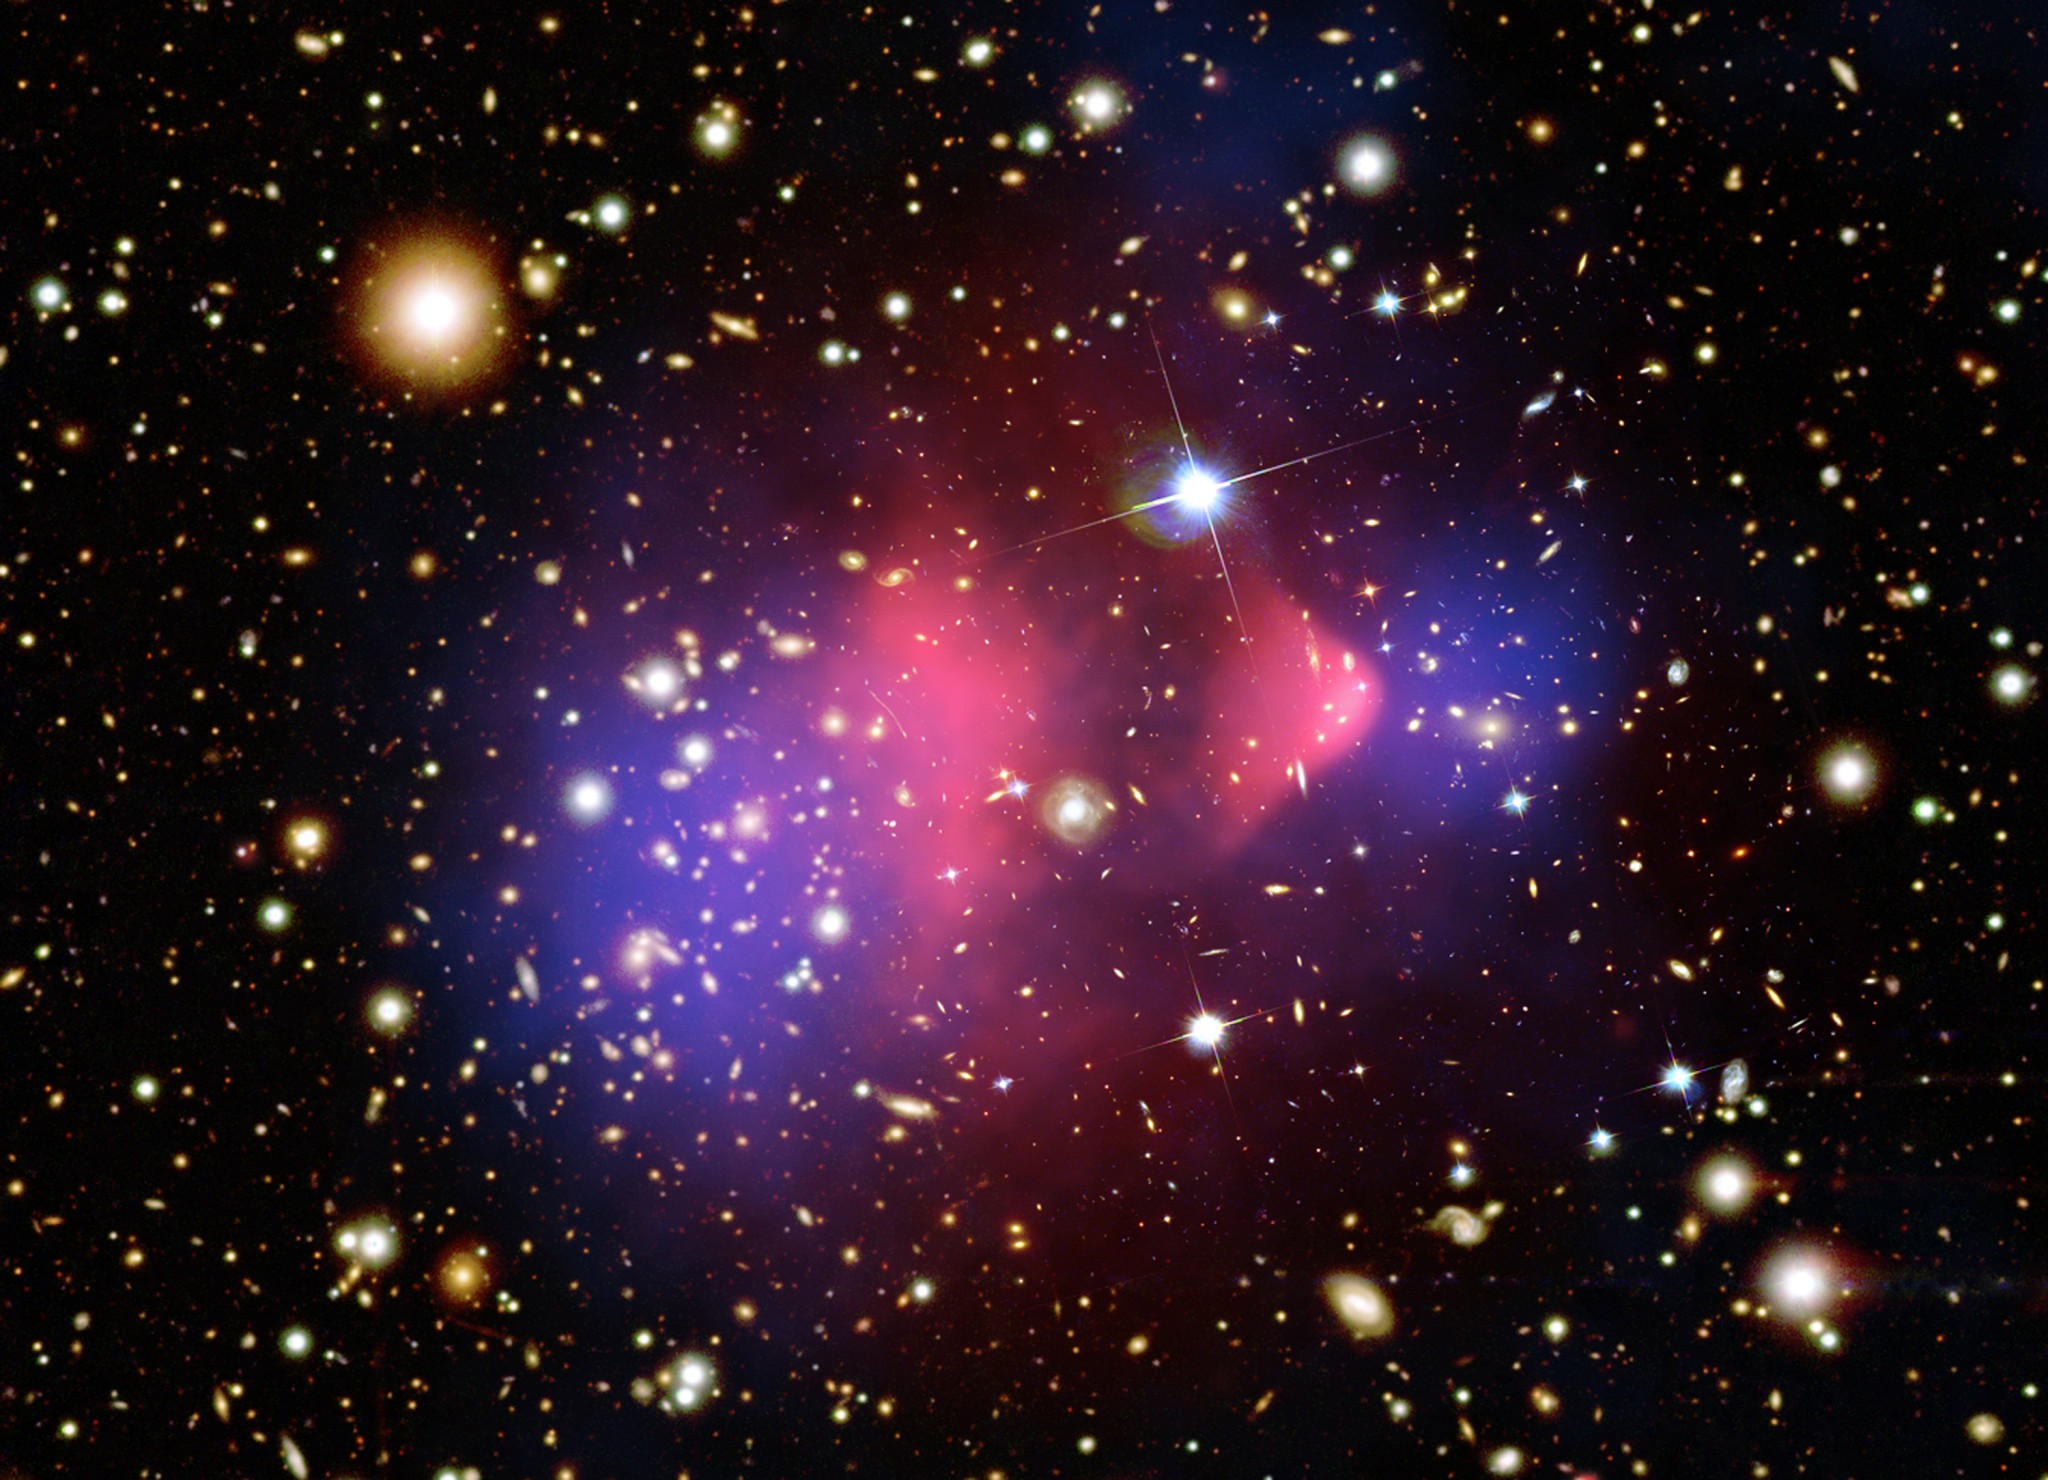
\includegraphics[width=0.95\textwidth]{images/bulletcluster.eps}
      \caption[The Bullet Cluster]{
        The Bullet Cluster~\cite{bullet_cluster_combined_image}.
        The blue clouds indicate the graviational lensing mass~\cite{bullet_cluster}, the red represents two clouds of ionized baryons emitting x-rays~\cite{bullet_cluster_chandramap}.
        The remaining stars and galaxies are imaged in the optical spectrum~\cite{bullet_cluster_composite}.}
      \label{fig:bullet}
    \end{figure}

    Followup studies have also been done of other galaxy clusters {\color{red}(and?? -Orel)}.

    {\color{red}(Mass to light ratios?? there is this paper \url{http://iopscience.iop.org/article/10.1086/303805/pdf}, but its the M/L field ratio, not just M/L)}

    In the second method, the velocity of different galaxies in a cluster can be measured.
    By comparing the velocities of different galxies in a cluster, the contained mass within the cluster can be measured.
    {\color{red}(Should be expanded (had to look it up to understand which effect you are referring to). -Orel ??)}

  \subsection{Scales of $10^{26}\:\text{m}$ : The Observable Universe}\label{dm_universe}
    %\subsection{Inter-Cluster Scale}
    % age of universe (13.82*10^9 years * speed of light) = 1.307*10^26m
    At the largest scale of the universe, $\nicetilde 10^{26}$m, the Cosmic Microwave Background (CMB) has been used to measure the total amount of Dark Matter in the universe.
    By looking at the structure of the CMB, the structure of the universe and its particle populations can be studied, including how they developed and changed from the big bang to the present day.
    Closer to the big bang, there was a point in time referred to as the 'freezout'.
    Before that time, the universe was a quark-gluon plasma {\color{red}and other particles (If you mention other particles, they should probably be named. -Orel ??)}, and the temperature was too hot to allow baryons to exist for any long period of time.

    % borrow dark matter-related events from this chart?
    % https://en.wikipedia.org/wiki/Chronology_of_the_universe
    \begin{table}[h]
      \centering
      \caption{
        Key events during the development of the universe.
        The Time column is the age of the universe at that event.
        The Temperature column is the universe's average temperature at that time.
        The Distance column is how far light could have traveled in that time, if it started at the beginning of the universe and travelled at present-day $c$.
        {\color{red}Idea from \url{http://www.th.physik.uni-bonn.de/drees/non\_ac/presentation\_Narimani.pdf} , slide 10, CREDIT THIS!!}
        {\color{red}(Source remaining values??)}
        {\color{red}(If a term is mentioned here, it needs to be explained!! ??)}
        % see http://www.sciencedirect.com/science/article/pii/S0370157304003515 page 286 for more info
        % see https://arxiv.org/pdf/hep-ph/0602002.pdf
        % maybe check PDG?
        % http://www.particleadventure.org/history-universe.html
      }
      % Space column is just Time column * 3e8 m/s
      \label{cosmo_events}
      \begin{tabular}{lccc}
        Event                                         & Time                    & Temperature               & Distance       \\
        \hline
        Inflation                                     & \SI{1e-34}{s}(?)        & ??                        & \SI{1e-26}{m}  \\
        Baryogenesis                                  & ??                      & ??                        & ??             \\
        EW phase transition                           & \SI{20}{ps}             & \SI{100}{\GeV}            & \SI{6}{mm}     \\
        Dark Matter Freeze-out                        & ??                      & ??                        & ??             \\
        QCD phase transition                          & \SI{20}{\mu.s}          & \SI{150}{\MeV}            & \SI{6}{km}     \\
        Neutrino decoupling                           & \SI{1}{s}               & \SI{1}{\MeV}              & \SI{3e8}{m}    \\
        Neutron freezout                              & \SI{1}{s}               & \SI{1}{\MeV}              & \SI{3e8}{m}    \\
        $\text{e}^+ - \text{e}^-$ annihilation        & \SI{6}{s}               & \SI{500}{keV}             & \SI{2e9}{m}    \\
        Big Bang nucleosynthesis                      & \SI{3}{min}             & \SI{100}{keV}             & \SI{5e10}{m}   \\
        Matter and radiation densities equal          & \SI{60}{kyr}            & \SI{0.75}{eV}             & \SI{6e20}{m}   \\
        Recombination                                 & \SIrange{260}{380}{kyr} & \SIrange{0.26}{0.33}{eV}  & \SI{3e21}{m}   \\
        Photon decoupling                             & \SI{380}{kyr}           & \SIrange{0.23}{0.38}{eV}  & \SI{3.6e21}{m} \\
        Reionization                                  & \SIrange{100}{400}{Myr} & \SIrange{2.6 }{7   }{meV} & \SI{2e24}{m}   \\
        Dark energy-matter equality                   & \SI{9}{Gyr}             & \SI{0.33}{meV}            & \SI{9e25}{m}   \\
        Present                                       & \SI{13.8}{Gyr}          & \SI{0.24}{meV}            & \SI{1e26}{m}   \\
      \end{tabular}
    \end{table}
    
    After that freezout, the temperature was low enough that baryon creation and annihilation rates plummited.
    Thus, the number of baryons that were in the universe at the freezout temperature determines how many baryons are in existance today, since there are no significant ways to destroy universe-scale quantities of baryons.
    This freezout left an imprint of its structure, where higher and lower densities of remaining baryons led to higher and lower densities of CMB photons.
    {\color{red}(This is not entirely accurate (the fraction of baryons to anti-baryons is too high to be explained as a simple statistical fluctuation which froze).
Also, it does not really explain how Dark Matter plays a role (you mention it in the next paragraph, but it is not explained). -Orel ?? )}

    From fitting this structure, the composition of the universe can be modelled.
    In terms of energy, 68.6\% of the universe {\color{red}is hypothesized to be Dark Energy (better scientific wording??)}, which causes almost all visible galaxies to accellerate away from the Milky Way.
    % 100% - ( 26.5% + 4.9 ) = 73.5% (from beginning of chapter)
    Another 4.9\% of the universe's energy is stored in baryonic matter, like protons and neutrons.
    The remaining 26.5\% of the universe's energy is contained in Dark Matter~\cite{planck2015}.

    Another important piece of evidence for the existance of Dark Matter is the abundance of Deuterium present in the universe.
    The amount of Deuterium that was left over from the big bang depends on the amount of baryons in the universe.
    The amount of baryons predicted by this is not enough to account for the total mass of the universe, thus it must exist in other (darker) particles.
    {\color{red}(The abundance of Deuterium is relevant for the argument of baryonic/non-baryonic Dark Matter. Meaning, it does not directly point to the existence of Dark Matter, but more suggests about its nature. It is a good point to bring up (and expand), but probably in a different section, no? -Orel ??)}
    Most theories of Dark Matter being trapped in cold dead stars, referred to as MAssivly Compact Halo Objects (MACHOs), have been abandoned due to this baryon limitation {\color{red}(cite??)}.

    Another measurement that depends heavily on the presence of Dark Matter is the rate at which galaxies form clumps.
    In the Sloan Digital Sky Survey (SDSS), the positions of 1.6 million galaxies, quasars, and stars are mapped~\cite{sdss_release}.
    By simulating the distribution of similar objects as the universe ages, only with a Dark Matter component does the universe form clumps that match SDSS observations.
  
    A much more detailed discussion on the evidence for Dark Matter can be read here \cite{DMPrimer}.
    {\color{red}(Unfortunately, this cannot really be done in a thesis (unlike a paper). A thesis needs to contain detailed explanations on its main subject. I guess you figured that already from all of my previous comments. -Orel ??)}
    {\color{red}(Take a few more ideas from that primer, explain them, then leave out the above line altogether)}

    {\color{red}(baryon acoustic oscillations?? \url{http://iopscience.iop.org/article/10.1086/466512/meta} )}
    
    
    {\color{red}(cmb temperature and polarization??)}
    

\section{$\Lambda$CDM Cosmology and the Standard Model}

  At the largest spatial scales, $\Lambda$CDM is the currently accepted model of cosmology.
  The $\Lambda$ refers to the density of dark energy, while CDM refers to Cold Dark Matter.
  $\Lambda$CDM models how the universe expanded from the big bang until the present day universe.
  This model predicts the different times particles froze out of the universe, and their resulting distributions.

  A large part of $\Lambda$CDM comes from measuring fluctuations in the Cosmic Microwave Background (CMB).
  In these fluctuations, a snapshot of the universe when it was 380,000 years old is preserved, providing many clues as to the development of the universe, including its age, energy content, structure, and expansion. 
  {\color{red}(You should explain what is learned from the CMB and how. -Orel ??)}
  This CMB snapshot also provides hints about the nature of Dark Matter, including some basic requirements for any potential Dark Matter candidate particle.

  \begin{figure}[ht]
    \includegraphics[width=0.95\textwidth]{images/cmb_skymap/cmb_skymap.eps}
    \caption[The Cosmic Microwave Background]{
      The cosmic microwave background temperature map of the universe \cite{wmap_skymap}, from 9 years of WMAP observations~\cite{wmap9year}.
      This image shows a temperature range of \SI{\pm200}{\mu{}Kelvin}.
    }
    \label{fig:cmb}
  \end{figure}

  The current paradigm of particle physics is called the Standard Model~\cite{standardmodel} {\color{red}(This is a random book on SM, is there a better one??)}.
  {\color{red}(I used 4 references for the original publications of electroweak theory and QCD, but I think a book is fine as well. If you want I can give you my references. -Orel ??)}
  It consists of groups of particles called quarks and leptons, as well as the bosons that mediate interactions between these particles.
  Quarks combine to form hadrons, like protons and neutrons, and mesons, while leptons consist of electrons, muons, {\color{red}tauons (is this right??)}, and their neutrino companions.

  At the forefront of {\color{red}these searches (what searches?? -Orel)} are particles predicted by Supersymmetry~\cite{Jungman:1995df}, (specifically Minimal Supersymmetric Standard Model, or MSSM~\cite{MSSM}), an extension to the Standard model.
  Much like how all particles have an anti-particle, in supersymmetry, each Standard Model quark, lepton, and boson, has a supersymmetric partner particle.
  Quarks and leptons have squarks and sleptons as their supersymmetric partners, while bosons have partners like photinos, gluinos, and charginos.
  While no evidence of supersymmetry has been discovered to date, it is still preferred due to its ability to predict physics across a large range energy scales, the holy grail of any Grand Unified Theory.
  

\section{Particle Dark Matter}\label{sec_particledm}

  Since all Standard Model particles have been eliminated as Dark Matter candidates {\color{red}(cite??)}, theoretically predicted particles are now the focus of many searches.

  One recently favored Standard Model Dark Matter candidate was the neutrino, due to its numerous nature and lack of interaction with the strong and electromagnetic forces.
  This was generally referred to as Hot Dark Matter, as neutrinos travel at relativistic speeds.
  However, it was eventually demonstrated that because of these relativistic speeds, neutrinos would diffuse out of their initial overdensities.
  This would result in large super-cluster-scale gravitational wells forming first, then cluster-scale wells, then galaxy-scale wells {\color{red}(what is the term for this?? hierarchicial formation? structure formation?)}.
  When observations are made of earlier times, the opposite is found: galaxy-scale gravitational wells form first, then cluster-scale wells, then super-cluster-scale wells in present times.
  As this is the opposite of what is expected for relativistic Dark Matter, neutrinos were ruled out as a Dark Matter candidate {\color{red}(cite??)}.
  % from this discussion: https://physics.stackexchange.com/questions/158319/why-are-neutrinos-ruled-out-as-a-major-or-even-sole-component-of-dark-matter
  
  {\color{red}(why neutralino??)}
  
  While the currently favored Dark Matter candidate is the neutralino, the lightest supersymmetric particle, a more general term for Dark Matter candidate particles that meets the conditions required by cosmology and particle physics is a WIMP, or Weakly Interacting Massive Particle.
  One of the major predictions from particle physics and cosmology is referred to as the "WIMP Miracle".
  In it, particle physics and cosmology separately predict that if Dark Matter is WIMP, it should have a velocity-averaged cross section of around \SI{3e-27}{cm$^3$s$^{-1}$}, though each field comes to this value by very separate math. {\color{red}(cite??)}
  {\color{red}(It's not exactly math, there is some physical constraints in it. Can you find a better way of explaining it?? -Orel)}

  In the 1990s, supersymmetry predicted the existance of a WIMP-like particle with a {\color{red}cross section (cross section is always 2 words!??)} of around \nicetilde \SI{3e-26}{cm$^2$}~\cite{Jungman:1995df}.
  % $3*{10}^{-26}\ {\textrm{cm}}^{2}$
  {\color{red}(And what happened since the 90s?? -Orel)}
  {\color{red}(Also, here is says $10^{-26}$ and before it said $10^{-27}$, intentional?? -Orel )}
  What made this WIMP particle a more promising candidate is that several cosmological problems can also be solved by a weakly-interacting GeV-TeV mass particle.
  {\color{red}What were these cosmological problems that were fixed??}
  Thus, two separate fields of physics recognized that they both were looking for a WIMP-like particle within the same mass and cross section range.

  In $\Delta$CDM cosmology, the relic density is all of the leftover Dark Matter particles after the universe became too cold to produce more Dark Matter particles.

  {\color{red}One or two more sentences on the relic density??}

  There are other potential Dark Matter candidates, both as other particle types or as modifications to other areas of physics, but they are not explored in this thesis.
  See Ref. \cite{DMPrimer} for more a more detailed discussion.



